\documentclass{article}
\usepackage[utf8]{inputenc}
\usepackage[english, swedish]{babel}

\usepackage{cite}
\usepackage{caption}
\usepackage{graphicx}
\usepackage{float}
\usepackage{textcomp}

\usepackage{listings}
\usepackage{color}
 
\definecolor{codegreen}{rgb}{0,0.6,0}
\definecolor{codegray}{rgb}{0.5,0.5,0.5}
\definecolor{codepurple}{rgb}{0.58,0,0.82}
\definecolor{backcolour}{rgb}{0.95,0.95,0.92}
 
\lstdefinestyle{mystyle}{
    backgroundcolor=\color{backcolour},   
    commentstyle=\color{codegreen},
    keywordstyle=\color{magenta},
    numberstyle=\tiny\color{codegray},
    stringstyle=\color{codepurple},
    basicstyle=\footnotesize,
    breakatwhitespace=false,         
    breaklines=true,                 
    captionpos=b,                    
    keepspaces=true,                 
    numbers=left,                    
    numbersep=5pt,                  
    showspaces=false,                
    showstringspaces=false,
    showtabs=false,                  
    tabsize=2
}

\lstset{style=mystyle}

\usepackage[yyyymmdd]{datetime}
\renewcommand{\dateseparator}{-}

\usepackage{graphicx}
\graphicspath{ {images/} }

%For headers & footers
\usepackage{fancyhdr}
\pagestyle{fancy}
\lhead{
\includegraphics[scale=0.2]{Logo}}
\chead{Kartrobot}
\rhead{\today}

\lfoot{Konstruktion med mikrodatorer}
\rfoot{Grupp 3}

\usepackage{titlesec}

\setcounter{secnumdepth}{4}

\titleformat{\paragraph}
{\normalfont\normalsize\bfseries}{\theparagraph}{1em}{}
\titlespacing*{\paragraph}
{0pt}{3.25ex plus 1ex minus .2ex}{1.5ex plus .2ex}

\renewcommand{\headrulewidth}{0.4pt}
\renewcommand{\footrulewidth}{0.4pt}


\title{Efterstudie}
\author{Patrik Sletmo}
\date{\today}

\selectlanguage{swedish}

\begin{document}

\thispagestyle{empty}

{
\sffamily
\centering
\large


{\huge 
Efterstudie
}

{\large
Patrik Sletmo
}

{\large
Version 1.0
}

\vspace{3.5cm}

Status
\begin{table}[H]
\centering
\begin{tabular}{ | c | c | c | }
\hline
-- & Patrik Sletmo & 2016-12-XX \\
\hline
\end{tabular}
\end{table}
}
\clearpage

\vspace*{\fill}
{
\sffamily
\centering
\large


{\huge
Projektidentitet
}

{\large
Grupp 3, 16/HT, KarToffel \\ Linköpings tekniska högskola, ISY
}

\vspace{0.5cm}

\begin{table}[H]
\centering
\begin{tabular}{ | c | c | c | c |}
\hline
Namn & Ansvar & Telefon & E-post \\
\hline
Patrik Sletmo & Projektledare & 070 783 57 61 & patsl736@student.liu.se \\
\hline
Rebecca Lindblom & Utvecklare & 073 436 40 79 & rebli156@student.liu.se \\
\hline
Matildha Sjöstedt & Utvecklare & 070 515 84 11 & matsj696@student.liu.se \\
\hline
Sebastian Callh & Utvecklare & 073 820 46 64 & sebca553@student.liu.se \\
\hline
Anton Dalgren & Utvecklare & 076 836 51 56 & antda685@student.liu.se \\
\hline
Matilda Dahlström & Utvecklare & 070 636 33 52 & matda715@student.liu.se \\
\hline
\end{tabular}
\end{table}
}

\begin{center}
\textbf{Hemsida}: https://github.com/SebastianCallh/kartoffel-tsea29
\end{center}

\begin{center}
\textbf{Kund}: Mattias Krysander, 013 - 28 2198 , matkr@isy.liu.se
\end{center}

\begin{center}
\textbf{Kursansvarig}: Tomas Svensson, 3B 528, +46 (0)13 28 1368, tomas.svensson@liu.se \\
\textbf{Handledare}: Anders Nilsson, 3B 512, +46 (0)13 28 2635, anders.p.nilsson@liu.se
\end{center}
\vspace*{\fill}
\clearpage

\renewcommand*\contentsname{Innehållsförteckning}
\tableofcontents

\clearpage
\section{Tidsåtgång}
Det var med stor osäkerhet vi gjorde vår första tidplan i det planerande skedet. Efter att ha reviderat tidplanen säkert fem gånger kom vi fram till en plan som vi åtminstone var lite säkrare på men under projektets gång visade det sig hur svårt det är att faktiskt lyckas göra en bra uppskattning av tidsåtgången i ett projekt.

\subsection{Arbetsfördelning}
Under projektets tidiga skede då vi byggde upp hårdvaran delades arbetet in i de olika delsystemen (huvudenhet, sensorenhet, styrenhet) för olika aktiviteter vilka arbetades på i par om två. Allt eftersom projektet fortskred övergick arbetet främst till att skriva Python-kod på huvudenheten och arbetet delades då in i olika mjukvarumoduler. Vem som gjort vad har genom hela projektet styrts av intresse och kompetens.

\subsection{Tidsåtgång jämfört med planerad tid}
Arbetet med designspecifikationen innan beslutspunkt 3 gick betydligt snabbare än planerat vilket gav oss mer tid inför beslutspunkt 5. Tidsåtgången för själva konstruktionen underskattades dock.

\begin{table}[H]
\centering
\caption{En tabell över projektets tidsåtgång.}
\begin{tabular}{ | c | c | c | }
\hline
Fas & Planerad tid i timmar & Använd tid i timmar \\
\hline
Före & 83 & 52 \\
\hline
Under & 851 & 922 \\
\hline
Efter & 26 & 16 \\
\hline
\end{tabular}
\label{table:tidsatgang}
\end{table}
\ \\


\clearpage
\section{Analys av arbete och problem}
Under konstruktionens inledande fas arbetade gruppen i väldigt separerade grupper med olika implementationer. Arbetet gick under den här perioden bra, men när olika funktionalitet skulle integreras uppstod problem och tiden spenderad på felsökning ökade markant. Efter att gruppen lyckats integrera all funktionalitet spenderades även en signifikant del av den återstående tiden med att testa olika metoder för hur vi filtrerade sensorvärden och på att finslipa regleringen. Det var ibland svårt att få perspektiv på hur ändringarna som gjordes skulle påverka robotens prestation, men efter en tid så löste även det problemet sig.

\subsection{Vad hände under de olika faserna (bra/dåligt/orsak)?}
I före-fasen flöt arbetet på bra, med interna deadlines innan de faktiska. Sjukdom påverkade arbetet negativt, men gruppen levererade ändå enligt plan. När under-fasen väl startade tilltog gruppens entusiasm då fokus flyttades från att skriva dokumentation till att vira och koda. Den här entusiasmen höll i sig fram till det att uppstod problem med integration av olika undergruppers moduler, då stämningen försämrades avsevärt, främst på grund av dålig kommunikation, vilket gjorde integrationen svårare än den hade behövt vara. Efter en lyckad leverans lades endast tid på att sammanställa detta dokument.

\subsection{Hur vi arbetade tillsammans (ansvar, beslut, kommunikation etc.)?}
I början av projektet hade vi en rätt så ojämn och krånglig ansvarsfördelning. Vi delade inte ut några specifika ansvarsområden förutom till projektledaren som hade det mesta ansvaret och även ansvarade för all dokumentation. När man påbörjade en aktivitet blev man direkt ansvarig för vad som gjordes där och vilka beslut som fattades kring den - på gott och ont. Vi strävade efter att alla skulle få fatta beslut kring vad de arbetade på för tillfället men det visade sig bara bli rörigt och inkonsekvent. I efterhand skulle det vara bättre att dela upp ansvaret för de olika modulerna över projektets medlemmar och låta beslutsfattningen göras av den eller de ansvariga.
\newline\newline
På grund av den här ansvarsfördelen behövdes beslut aldrig riktigt kommuniceras uppåt utan det gick att implementera sin funktionalitet och sedan direkt påbörja nästa aktivitet. Det här ledde till stor förvirring när resten av gruppen sedan skulle försöka förstå sig på funktionen i senare aktiviteter och det togs även beslut som gjorde att onödig funktionalitet implementerades, vilket tog mycket tid från projektet. När vi till slut fick möjlighet att åtgärda det här kommunikationsproblemet var vi för långt in i projektet för att applicera den tidigare nämnda lösningen som innebar olika ansvarsområden utan vi behövde ett annat angreppssätt. Lösningen blev att introducera en ny kommunikationskanal där vi efter varje avslutat pass eller arbetsdag skrev en text som beskrev vad vi gjort för något. Förutom att ge en bättre förståelse för projektets olika delar gav det också alla en insikt i vad som hände i projektet och vilka framsteg som gjordes. Hela gruppen upplevde att kommunikationen fungerade bättre efter detta beslut tagits.

\subsection{Hur använde vi projektmodellen?}
Projektmodellen LIPS användes flitigt i den förberedande fasen för projektet. Vi skrev all dokumentation enligt modellens mallar och följde dess beslutspunkter. Under projektets gång efter vi passerat beslutspunkt 4 så blev det inte lika självklart att följa projektmodellen och vi applicerade egentligen inget av modellens arbetssätt.
\newline\newline
Det fanns aldrig någon riktig verifiering av de aktiviteter vi genomförde utan de bedömdes som färdiga av de gruppmedlemmar som genomförde dem. Genom att faktiskt verifiera aktiviteter med någon annan gruppmedlem och verkligen testa funktionaliteten hade vi antagligen kunnat undvika många problem som orsakats av att funktioner inte fungerat för alla fall de senare skulle utsättas för. När vi bestämde en aktivitet som avklarad och påbörjade nästa för att vara i fas med tidplanen sköt vi bara problemet längre fram.

\subsection{Hur fungerade relationen med beställaren?}
Gruppen upplever inte att den haft någon nära relation med beställaren, men att han varit lätt att få tag på och att kommunikationen har fungerat väl. Kritiken som gavs på den tekniska dokumentationen uppskattades. 

\subsection{Hur fungerade relationen med handledaren?}
Handledaren fanns oftast till hands när vi behövde ställa frågor, vilket var en användbar resurs då gruppen konstruerade hårdvaran. Gruppen upplevde inte ett så stort behov att att ställa frågor, men är mycket nöjd med den hjälp som givits. Handledaren har visat intresse även då gruppen inte behövt något stöd.

\subsection{Tekniska framgångar/Problem}
Att arbeta med hårdvara på det sättet vi gjort innebär betydligt fler svårigheter än vad vi är vana vid när man endast arbetar med mjukvara. Att behöva korrigera för och behandla verklighetens alla avvikelser har varit en svår uppgift och orsakat många av gruppens problem men det har även lett till nya lösningar som vi är mycket stolta över.

\subsubsection{Mätvärden från laser}
Vid första leveransen upplevdes inte positionsbestämningen fungera konsekvent, vilket visade sig bero på två olika saker. 
\begin{figure}[H]
\centering
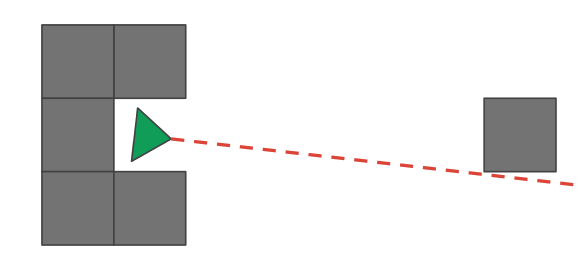
\includegraphics[scale=0.5]{wrongly_positioned_laser}
\caption{En bild på hur fel positionering påverkar lasern.}
\label{fig:wrongly_positioned_laser}
\end{figure}
\ \\
För det första kunde robotens lasersensor ge orimliga värden helt spontant och för det andra så positionerades den inte korrekt efter svängar, vilket ledde till att den på längre avstånd kunde får markanta felläsningar. Se figur~\ref{fig:wrongly_positioned_laser} för en illustration på detta.
\newline\newline
Att lasersensorn kunde ge konstiga värden berodde förmodligen på något fel på låg nivå, antingen på robotens I2C-buss eller till och med hårdvara. Detta felsöktes dock inte eftersom det uppskattades ta för lång tid, och fokus lades på att filtrera laservärden på ett sätt som skulle eliminera dessa felaktiga mätningar. Detta gjordes främst genom att ignorera laservärden som skiljde sig för mycket från tidgare värden. Om felet ej hade uppstått hade flertalet dagar kunnat sparas in under projektets sista veckor.
\newline\newline
Att roboten kunde ställa sig snett berodde på dess navigeringslogik, vilken fick förbättras. Navigationslogiken är programmerad som en tillståndsmaskin, och för att lösa problemet lades ett nytt tillstånd till som roboten går in i efter varje sväng, där den korrigerar sin riktning. På så sätt kunde det säkerställas att roboten alltid stod parallelt med väggen på höger sida efter en sväng och att lasern träffade där den skulle. När problemet väl upptäcks åtgärdades det på bara några timmar, men det hade länge legat och spökat under testkörningar. Det är svårt att urskilja vilket problem som påverkade när, men även det här felet kan ha kostat gruppen flera dagar av felsökning.

\subsubsection{Utveckling av Bluetooth}
Under utvecklingen av mjukvaruklienten samt robotens uppkoppling mot den, upplevdes stor tidsåtgång på dess aktiviteter. Planerad tid för Bluetoothkommunikation samt mjukvaruklient var ungefär 40 timmar, och den lagda tiden hamnade på nästan 200 timmar. 
\newline\newline
Då både server- och klientsidan utvecklades i Python användes biblioteket Pybluez för Bluetoothuppkopplingen. Orsaker till att detta problem uppstod var dels att detta bibliotek var dåligt dokumenterat, underskattning av planerad tidsåtgång, vissa uppgifter föll mellan de specificerade aktiviteterna och blev inbakade i de ursprungliga aktiviteterna, ingen tidigare kunskap om nätverksprogrammering eller processhantering i Python samt dålig kommunikation inom gruppen för planering av nivån på lösningarna. 

\subsubsection{Uppkoppling över trådlöst nätverk}
När vi planerade gruppens arbetsflöde gjorde vi antagandet att vi likt en bärbar dator kunde koppla upp robotens huvudenhet, som bestod av en Raspberry Pi, på det trådlösa nätverket \textit{eduroam}. Antagandet var egentligen inte inkorrekt, vi kunde koppla upp roboten på nätverket och nå den från en annan dator på samma nätverk. Det som orsakade problem var stabiliteten hos uppkopplingen.
\newline\newline
Det felaktiga antagandet som orsakade vårt designfel var att anslutningen från en Raspberry Pi skulle erbjuda samma stabilitet som för en bärbar dator. Problemet med Raspberry Pi:n är att den endast har en antenn för 2.4 GHz-bandet, som utöver det också är väldigt liten. Detta ledde till att vi fick svårigheter att bibehålla en uppkoppling mot enheten och ofta var tvungen att försöka återansluta. Inte allt för sällan hade IP-adressen på nätverket förändrats sen senaste gången vi försökte ansluta och vi var därför tvungna att vänta på att robotens display skulle uppdateras med den nya adressen - något som bara sker en gång per minut.
\newline\newline
Om en skulle uppskatta antalet timmar som förlorats på grund av problem med uppkopplingen har det rört sig om ett par tiotal timmar bortkastad tid. Vad som egentligen borde gjorts så fort vi upptäckte att det här var ett problem hade varit att dela mobilnätverket från en mobil där både robot och uppkopplad dator hade kunnat anslutas. Under projektets gång ignorerade vi istället en möjlig lösning och lät problemet ligga kvar och ta upp tid. Detta beror på att alla var fokuserade på att få andra saker att fungera så det här var aldrig något som prioriterades.

\clearpage
\section{Måluppfyllelese}
Gruppen har inte satt upp några mål att uppnå i projektet. Det som fokuserades på under projektet var att klara kursen och de delmoment i projektet som detta grundades på. Med det sagt har vi fått flera viktiga erfarenheter från projektets gång som vi kan ta med oss till senare projekt.

\subsection{Vad har uppnåtts?}
Vi har lyckats producera en robot som uppfyller alla de krav vi satt upp innan projektets början. Dessutom så innehåller systemet funktionalitet som vi som grupp kanske inte anser nödvändigt för robotens funktion men uppfyller våra egna ambitioner. Vad som framför allt uppnåtts under projektet är att vi lärt oss vikten av bra kommunikation och att kunna arbeta tillsammans på ett strukturerat vis. Trots alla tekniska problem vi stött på så har kommunikationen varit den del av projektet som betytt mest för projektets framgång.

\subsection{Hur fungerade leveransen?}
Kvällen innan mötet för beslutspunkt 5 hade roboten konsekvent klarat en bana, men den var helt klart inte konsekvent nog då den vid leverans inte klarade banan en enda gång. En omleverans bokades in tre dagar senare, och på den tiden lyckades gruppen identifiera och lösa felen som lett till robotens inkonsekventa beteende. Vid det kompletterande mötet för beslutspunkt 5 klarade roboten fyra av fyra körningar, varav två kördes på en helt okänd bana. Gruppen är mycket nöjd med robotens kvalitet vid leverans.

\subsection{Hur har studiesituationen påverkat projektet?}
Då nästan hela gruppen har haft olika scheman, deltidsarbetat och varit aktiva i tidskrävande studentföreningar har schemaläggning varit en utmaning, och många timmar har lagts på kvällstid och helger. 

\clearpage
\section{Sammanfattning}
Att få genomföra det här projektet har gett oss mycket lärdom och erfarenheter, både om att arbeta med hårdvara och vilka svårigheter det innebär, men vi har fått minst lika mycket kunskap från grupparbetet. Det har funnits stunder då projektet har gått riktigt bra och det finns stunder när allt känts hopplöst. Det sägs att man inte lär sig något utan att misslyckas och även om vi till slut lyckades ta fram en välfungerande och till och med vinnande robot har det funnits många felsteg i projektet där vi lärt oss mycket vi kan ta med oss till kommande arbeten. Samtidigt som det är tråkigt att arbetet stundvis inte alls fungerat bra ser vi det som en möjlighet till förbättring och vi är glada att ha erfarenheterna i bagaget till kandidatarbetet i vår.

\subsection{De tre viktigaste erfarenheterna}
\subsubsection{Kommunikation är viktigt}
Det är väldigt svårt att genomföra ett projekt utan bra kommunikation inom gruppen. Samtidigt som det tar tid att lägga upp ett bra arbetsflöde där alla är med på vad som händer och är nöjda med vad hen får säga till om i projektet tar det mångfaldigt längre tid att genomföra projektet med ett dåligt kommunikationsflöde. Det går att skapa otroligt bra tekniska lösningar, men utan bra kommunikation så bidrar inte en sådan lösning med särskilt mycket mer än ett halvdant alternativ.
\newline\newline
Att ständigt påverkas av konsekvenserna från dålig kommunikation påverkar stämningen i en grupp negativt. Vi upplevde att samarbetet inte alls fungerade i början av projektet och att gruppens medlemmar blev upprörda på varandra på grund av det här. Problemet vi upplevde var att vi inte såg helheten i varför det blev som det blev utan fokuserade på varje enskild sak istället för att inse att orsaken låg i hur vi arbetade. När vi senare anpassade vårt sätt att arbeta på genom att kommunicera tydligare vad som hände i projektet bidrog det till att samarbetet gick lättare och gruppen fick en bättre överblick i hur vi låg till. Det är viktigt att inkludera alla i vad som händer så att inte en viss diskussion tas mellan två personer och sedan antas som accepterad och känd av resten av gruppen.

\subsubsection{Gör inte saker för avancerade}
Flera gånger under projektets gång hände det att vi byggde allt för avancerade lösningar till problem som hade kunnat lösas på ett mycket simplare vis. Utan att analysera vad för funktionalitet som faktiskt krävdes påbörjades komplicerade lösningar som förvisso utökade funktionaliteten men som inte löste något egentligt problem vi upplevde. Två exempel på det här är abstraktionen och protokollet som användes för I2C-bussen samt Bluetooth-servern.
\newline\newline
Det gjordes antaganden om att I2C-bussen inte klarade av att leverera den data vi behövde kommunicera mellan enheterna och att vi behövde lägga på ett abstraktionslager (som sedan utökades till två) för att få dataflödet att fungera korrekt. I efterhand så fanns det ingen anledning alls att implementera all den här extra funktionaliteten utan problemet hade kunnat lösas genom att följa I2C:s standardprotokoll och på så sätt spara in många timmar samt underlätta förståelsen.
\newline\newline
I fallet med Bluetooth så byggdes en lösning som erbjöd redundant funktionalitet samt möjligheten att ansluta till roboten samtidigt som dess kartläggningsmjukvara inte var igång. Vad som senare upptäcktes var att den här redundansen inte alls behövdes då vi ändå var tvungna att starta om både kartläggningsmjukvaran och mjukvaruklienten varje gång vi återigen ville påbörja kartläggningen.

\subsubsection{Struktur och planering}
Troligtvis hade beslut att inte bygga den här avancerade funktionaliteten kunnat fattas om strukturen i projektet sett annorlunda ut. Det fanns ingen bra beslutshierarki i vår grupp utan som tidigare förklarat lät vi de ansvariga för varje aktivitet fatta deras egna beslut. Att faktiskt planera en bra hierarki och struktur hade underlättat situationer som dessa och även avlastat ansvaret från projektledaren.
\newline\newline
Vi hade i princip ingen planering för arbetet förutom tidplanen. Det fanns inget sätt att avgöra hur färdig en aktivitet var eller när nästa egentligen var redo att påbörjas, även om vi hade sagt att ingen aktivitet skulle påbörjas utan att den gick att testa till 100\%. Eftersom vi gick in i projektet med visionen om att det var viktigt att följa den tidplan vi satt upp prioriterade vi att påbörja nya aktiviteter över att avsluta gamla aktiviteter korrekt. Det här tillsammans med att det fanns dålig möjlighet att arbeta parallellt i projektet gjorde att arbetet stundvis blev väldigt hektiskt. Tyvärr är det svårare att arbeta parallellt med en fysisk produkt som endast återfinns i ett exemplar och på grund av detta hade det behövts läggas mer tid i den här delen av den planerande fasen. Många av problemen vi erfarde under projektet hade kunnat undvikas genom att lägga mycket mer tid på planering och analysera lösningar i det planerande skedet istället för att senare drabbas av dess konsekvenser och behöva tänka om först då.

\subsection{Goda råd till de som ska utföra ett liknande projekt}
Det är svårt att få med alla erfarenheter och att bestämma vilka råd som är värda att ta vidare. Det här är de råd vi anser vara viktigast att följa för att undvika de fallgropar vi stött på:

\begin{itemize}
    \item Kommunicera mera! Det är svårt att lägga för mycket tid på just kommunikation. Se till att alla vet var som händer i alla delar av projektet, varje dag!
    \item Planera upp en vettig struktur och hierarki inom gruppen istället för att hålla hierarkin mestadels platt med en huvudansvarig och resten utvecklare.
    \item Använd versionshantering för både kod och dokumentation. Att kunna backa till ett tidigare skede av projektet är otroligt tacksamt när en stöter på problem.
    \item Gå sakta fram i projektet och överskatta tidsåtgången. Saker tar längre tid än man tänkt från början, särskilt när man arbetar med hårdvara och nya tekniker.
    \item Se till att saker fungerar med tillräckligt hög pålitlighet innan ni går vidare. Att behöva backa tillbaka flera veckor för att en grundläggande funktion inte fungerar som den ska i en viss situation tar mycket tid.
    \item Samtidigt som det bidrar till en stabilare robot är det sjukt våghalsigt att ha krav på formen ``roboten ska klara 3 av 3 körningar''.
    \item Lös problem i arbetsflödet direkt! Finns det något som gör att ni ofta lägger onödigt mycket tid eller som påverkar gruppens samarbete lönar det sig att skjuta upp allt annat för att behandla det här problemet direkt. Att skjuta på problemet gör bara att det tar upp ännu mer tid!
\end{itemize}

\nocite{*}
\bibliography{efterstudie}{}
\bibliographystyle{plain}

\end{document}
